%%%%%%%%%%%%%%%%%%%%%%%%%%%%%%%%%%%%%%%%%
% Wenneker Assignment
% LaTeX Template
% Version 2.0 (12/1/2019)
%
% This template originates from:
% http://www.LaTeXTemplates.com
%
% Authors:
% Vel (vel@LaTeXTemplates.com)
% Frits Wenneker
%
% License:
% CC BY-NC-SA 3.0 (http://creativecommons.org/licenses/by-nc-sa/3.0/)
% 
%%%%%%%%%%%%%%%%%%%%%%%%%%%%%%%%%%%%%%%%%

%----------------------------------------------------------------------------------------
%	PACKAGES AND OTHER DOCUMENT CONFIGURATIONS
%----------------------------------------------------------------------------------------

\documentclass[11pt]{scrartcl} % Font size

%%%%%%%%%%%%%%%%%%%%%%%%%%%%%%%%%%%%%%%
% Wenneker Assignment
% Structure Specification File
% Version 2.0 (12/1/2019)
%
% This template originates from:
% http://www.LaTeXTemplates.com
%
% Authors:
% Vel (vel@LaTeXTemplates.com)
% Frits Wenneker
%
% License:
% CC BY-NC-SA 3.0 (http://creativecommons.org/licenses/by-nc-sa/3.0/)
% 
%%%%%%%%%%%%%%%%%%%%%%%%%%%%%%%%%%%%%%%%%

%----------------------------------------------------------------------------------------
%	PACKAGES AND OTHER DOCUMENT CONFIGURATIONS
%----------------------------------------------------------------------------------------
\usepackage{xcolor}   % for \textcolor
\usepackage{comment}

\usepackage{amsmath, amsfonts, amsthm} % Math packages

\usepackage{listings} % Code listings, with syntax highlighting
\usepackage{verbatim} % Directly from txt file

\usepackage[english]{babel} % English language hyphenation
\usepackage{tikz} 
\usepackage{neuralnetwork} 
\usepackage{graphicx} % Required for inserting images
\graphicspath{{Figures/}{./}} % Specifies where to look for included images (trailing slash required)
\usepackage{setspace}  % allows linespacing changes
\usepackage{tabularx} % for tables

\usepackage{booktabs} % Required for better horizontal rules in tables

\numberwithin{equation}{section} % Number equations within sections (i.e. 1.1, 1.2, 2.1, 2.2 instead of 1, 2, 3, 4)
\numberwithin{figure}{section} % Number figures within sections (i.e. 1.1, 1.2, 2.1, 2.2 instead of 1, 2, 3, 4)
\numberwithin{table}{section} % Number tables within sections (i.e. 1.1, 1.2, 2.1, 2.2 instead of 1, 2, 3, 4)

\setlength\parindent{0pt} % Removes all indentation from paragraphs

\usepackage{enumitem} % Required for list customisation
\setlist{noitemsep} % No spacing between list items

%----------------------------------------------------------------------------------------
%	DOCUMENT MARGINS
%----------------------------------------------------------------------------------------

\usepackage{geometry} % Required for adjusting page dimensions and margins

\geometry{
	paper=a4paper, % Paper size, change to letterpaper for US letter size
	top=2.5cm, % Top margin
	bottom=3cm, % Bottom margin
	left=3cm, % Left margin
	right=3cm, % Right margin
	headheight=0.75cm, % Header height
	footskip=1.5cm, % Space from the bottom margin to the baseline of the footer
	headsep=0.75cm, % Space from the top margin to the baseline of the header
	%showframe, % Uncomment to show how the type block is set on the page
}

%----------------------------------------------------------------------------------------
%	FONTS
%----------------------------------------------------------------------------------------

\usepackage[utf8]{inputenc} % Required for inputting international characters
\usepackage[T1]{fontenc} % Use 8-bit encoding

\usepackage{fourier} % Use the Adobe Utopia font for the document

%----------------------------------------------------------------------------------------
%	SECTION TITLES
%----------------------------------------------------------------------------------------

\usepackage{sectsty} % Allows customising section commands

\sectionfont{\vspace{6pt}\centering\normalfont\scshape} % \section{} styling
\subsectionfont{\normalfont\bfseries} % \subsection{} styling
\subsubsectionfont{\normalfont\itshape} % \subsubsection{} styling
\paragraphfont{\normalfont\scshape} % \paragraph{} styling

%----------------------------------------------------------------------------------------
%	HEADERS AND FOOTERS
%----------------------------------------------------------------------------------------

\usepackage{scrlayer-scrpage} % Required for customising headers and footers

\ohead*{} % Right header
\ihead*{} % Left header
\chead*{} % Centre header

\ofoot*{} % Right footer
\ifoot*{} % Left footer
\cfoot*{\pagemark} % Centre footer
 % Include the file specifying the document structure and custom commands
\usepackage{hyperref}

%----------------------------------------------------------------------------------------
%	TITLE SECTION
%----------------------------------------------------------------------------------------

\title{	
	\normalfont\normalsize
	\textsc{Intelligent Robotics, Portland State University}\\ % Your university, school and/or department name(s)
	\vspace{25pt} % Whitespace
	\rule{\linewidth}{0.5pt}\\ % Thin top horizontal rule
	\vspace{20pt} % Whitespace
	{\huge HW4}\\ % The assignment title
	\vspace{4pt} % Whitespace
	{\large Eyebrow CNN Training}\\ % The assignment title
	\vspace{12pt} % Whitespace
	\rule{\linewidth}{2pt}\\ % Thick bottom horizontal rule
	\vspace{12pt} % Whitespace
}

\author{\LARGE Trenton Ruf} % Your name
\date{\normalsize \today} % Today's date (\today) or a custom date

\begin{document}
\maketitle % Print the title
%\renewcommand\thesubsection{\Alph{subsection}}
%\renewcommand\thesubsection{\Roman{subsection}}
%\doublespacing
%\singlespace
%\onehalfspacing
%\setstretch{1.25}

%\begin{doublespace}
%\end{doublespace}

%\vspace*{\fill}
%\clearpage
%\vspace*{\fill}


%\vspace*{\fill}
\renewcommand\thesubsection{\Roman{subsection}}

\section{Importing Data}
The dataset was split into 80\% Training and 20\% Validation. 
The only pre-processing done was a normalization of the image pixel values to be between 0 and 1.
This pre-processing was done "in model" though. 
This way when using the model later all I have to do is pass it a raw image and it will normalize it for me.

\section{Data Augmentation}
To make up for my small dataset I implemented four common data augmentation layers. The augmentation only applies to the training data, and only while training. These augmentations are a ±2\% random rotation, zoom, contrast, and a ±5\% random brightness. I did not apply the common image flip augmentation because then it couldn't tell the difference between left or right when only one eyebrow was raised.


\section{Model}
I added three convolutional layers followed by a 2x2 pooling layer. 
I've read that many computer vision researchers dislike pooling because it decreases the feature space, but implemented it because it should offer a real-time speed advantage for a trade-off in accuracy.
I then added a series of dropout layers and dense hidden layers before ending it with a softmax.
The output of the convolutions was flattened before the first dense layer to coalesce the features into a 1-D array.
I want to experiment more with the number of dense layers and their perceptron count. I will do that during the winter break before next term.
As it is the model is far larger than I want it to be, so I will decrease the number of perceptrons and convolutional filters in the future.

\section{Training}
The model was trained until its validation loss value no longer decreased after 15 epochs in a row. 
This was done with keras' early stopping feature. Since I don't have a dedicated GPU the training was very slow. 
It took over 40 hours to train this model. Another reason I want to try decreasing the number and size of the layers.

\section{Performance}

\begin{figure}[ht!] % [h] forces the figure to be output where it is defined in the code (it suppresses floating)
	\centering
	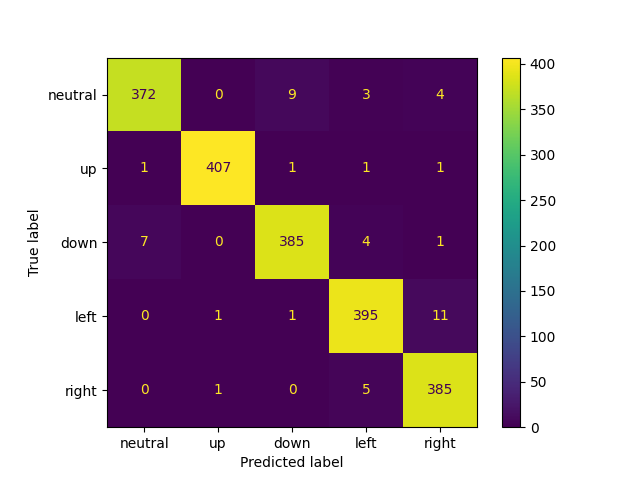
\includegraphics[width=0.8\columnwidth]{figures/confusionMatrix_RGB.png} 
	\caption{Confusion matrix}
\end{figure}

The model converged around 500 epochs at over 97\% accuracy on the validation data. It had the most trouble distinguishing between a couple categories. 
Neutral and down eyebrows was one. 
The distance covered by the eyebrows is the least between these two, so maybe that is the reason.
The other category pair that had difficulties was left and right.
This initially didn't make much sense to me because these should be the two that are the most different from each other since they are opposite. I believe the issue stems from the dataset rather than the model. 
When looking through the dataset manually I found quite a few pictures of left raised eyebrows that were actually right. 
I will remake the left and right portion of the dataset and train it again in the future.
\clearpage

\begin{figure}[ht!] % [h] forces the figure to be output where it is defined in the code (it suppresses floating)
	\centering
	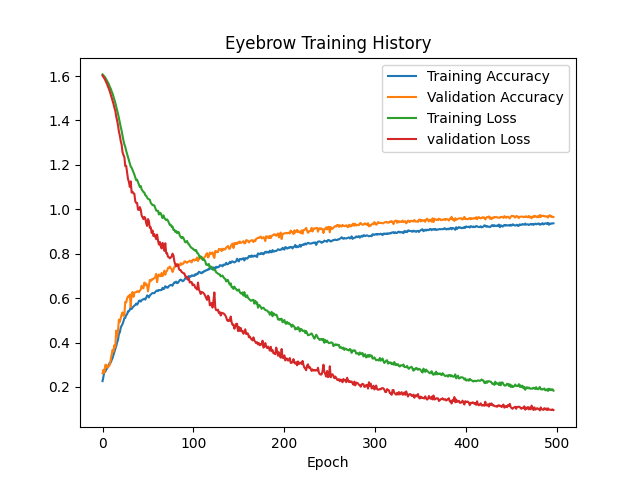
\includegraphics[width=0.8\columnwidth]{figures/trainingGraph_RGB.png} 
	\caption{}
\end{figure}

\section{future testing}
Along with decreasing the size of the model I want to do more accuracy comparisons with varying:
\begin{itemize}
	\item Data augmentation levels
	\item Dataset size 
	\item Un-even dataset distributions
	\item Color - RGB vs Grayscale
\end{itemize}

\clearpage

\section{code}

All files related to this project can be found at: 

\url{https://github.com/Trenton-Ruf/Intelligent_Robotics}

\lstinputlisting[
	caption= faceTrain.py, % Caption above the listing
	%label=lst:test, % Label for referencing this listing
	language=Python, % Use Perl functions/syntax highlighting
	frame=single, % Frame around the code listing
	breaklines=true,
	postbreak=\mbox{\textcolor{red}{$\hookrightarrow$}\space},	
	showstringspaces=false, % Don't put marks in string spaces
	numbers=left, % Line numbers on left
	numberstyle=\tiny, % Line numbers styling
	basicstyle=\footnotesize
	]{../../../faceCNN/faceTrain.py}

\end{document}

